\documentclass{book}
% Chinese
%\documentclass[UTF8, nofonts, mathptmx, 12pt, onecolumn]{article}
%\usepackage{xeCJK}
%\setCJKmainfont{SimSun}
\usepackage{amsmath}
\usepackage{amsfonts}
\usepackage{amssymb}
\usepackage{wasysym}
%\usepackage{ctex}
\usepackage{graphicx}
\usepackage{float}
\usepackage{geometry}
\geometry{a4paper,scale=0.8}
\usepackage{caption}
\usepackage{subcaption}
% \newcommand{\oiint}{\mathop{{\int\!\!\!\!\!\int}\mkern-21mu \bigcirc} {}}
\newcommand*{\dif}{\mathop{}\!\mathrm{d}}
\newcommand*{\md}{\mathop{}\!\mathrm{d}}
\newcommand*{\me}{\mathrm{e}}

\usepackage{parskip}
\setlength{\parindent}{0cm}

\usepackage{bm}
\let\Oldmathbf\mathbf
\renewcommand{\mathbf}[1]{\boldsymbol{\Oldmathbf{#1}}}
\let\eqnarray\align

\usepackage{authblk}
\author{Xiping Hu}
\affil{https://hxp.plus/}
\title{Analogue Electronics}
\date{}
\begin{document}
\maketitle
\tableofcontents

\chapter{绪论}

\section{教材}

\begin{itemize}
\item 龚云贵 yggong@hust.edu.cn 东七楼432
\item 《电动力学》(第三版) 郭硕鸿
\end{itemize}

\section{主要内容}

\begin{itemize}
\item 麦克斯韦方程组的逻辑推导和物理内涵
\item 静电及静磁的基本求解:格林函数、分离变量、镜像法
\item 电磁波的传播及其辐射
\item 电磁本质规律:规范不变性
\item 矢量、张量及四维时空观
\item 电磁作用量
\item 电磁学研究规律及方法
\end{itemize}



%%% Local Variables:
%%% mode: latex
%%% TeX-master: "Electro-Dynamics"
%%% End:

\chapter{Electromagnetic Theory and photons}

\section{Maxwell's Equation}

Faraday's Induction Law
\begin{equation*}
  \oint_{c} \vec{E} \cdot \md \vec{l} = - \dfrac{\md}{\md t} \iint \vec{B} \cdot \md \vec{S}
\end{equation*}

Gauss's Law
\begin{equation*}
  \oiint_{A} \vec{E} \cdot \md \vec{S} = \dfrac{1}{\varepsilon_{0}} \iiint_{v} \rho \md V 
\end{equation*}

\begin{equation*}
  \oiint_{A} \vec{B} \cdot \md \vec{S} = 0
\end{equation*}

Ampere's Circuital Law

\begin{equation*}
  \oint_{C} \vec{B} \cdot \md \vec{l} = \mu_{0} \iint_{A} \left( \vec{J} + \varepsilon_{0} \dfrac{\partial \vec{E}}{\partial t}  \right) \cdot \md \vec{S}
\end{equation*}

We can now take the derivatives of the 4 equations

\begin{equation*}
  \left\{
  \begin{aligned}
    \nabla \times \vec{E} &= - \dfrac{\partial B}{\partial t} \\
    \nabla \times \vec{B} &= \mu_{0} \varepsilon_{0} \dfrac{\partial \vec{E}}{\partial t}  \\
    \nabla \cdot \vec{E} &= \dfrac{\rho}{\varepsilon_{0}} \\
    \nabla \cdot \vec{B} &= 0
  \end{aligned}
  \right.
\end{equation*}

The Following Equation can be derived from Maxwell Equation above

\begin{equation*}
  \begin{aligned}
    \nabla^{2} \vec{E} = \mu_{0} \varepsilon_{0} \dfrac{\partial^{2} \vec{E}}{\partial t^{2}}\\
    \nabla^{2} \vec{B} = \mu_{0} \varepsilon_{0} \dfrac{\partial^{2} \vec{B}}{\partial t^{2}} 
  \end{aligned}
\end{equation*}

Coincidentally
\begin{equation*}
  c = \dfrac{1}{\sqrt{\mu_{0} \varepsilon_{0}}} 
\end{equation*}

Which indicates the speed of electromagnetic wave is the speed of light.

Furthermore, it can be seen that the electric field and magnetic field are transverse. They are perpendicular to each other. We assume the electric field is parallel to the y-axis.

\begin{equation*}
  \begin{aligned}
    E_{y} (x,t) = E_{0} \cos \left[ \omega \left( t - x/c  \right) + \varepsilon \right]
  \end{aligned}
\end{equation*}
According to Faraday's Law
\begin{equation*}
  \begin{aligned}
    \dfrac{\partial E_{y}}{\partial x} = - \dfrac{\partial B_{Z}}{\partial t}  
  \end{aligned}
\end{equation*}
We can calculate $B_{z}$

\begin{equation*}
  \begin{aligned}
    B_z = \dfrac{1}{c} E_{0} \cos \left[ \omega \left( t - x/c  \right) + \varepsilon \right]
  \end{aligned}
\end{equation*}
So that
\begin{equation*}
  \begin{aligned}
    E_y = c B_z
  \end{aligned}
\end{equation*}
When not in vacuum, similarly
\begin{equation*}
  \begin{aligned}
    E_y=vB_z \\
    v=\frac{1}{\varepsilon\mu}
  \end{aligned}
\end{equation*}

\section{Energy}

\begin{equation*}
  \begin{aligned}
    u_{E} &= \dfrac{\varepsilon_{0}}{2} E^{2} \\
    u_{B} &= \dfrac{1}{2\mu_{0}} B^{2} \\
    u_{E} &= u_{B} \\
    u &= u_{E} + u_{B} = \varepsilon_{0} E^{2} = \dfrac{1}{\mu_{0}} B^{2} \\ 
    S &= uc \\
    \vec{S} &= \dfrac{1}{\mu} \vec{E} \times \vec{B} \quad \mathrm{(Poynting Vector)}\\
    I &= \dfrac{1}{2} \varepsilon v E_0^2
  \end{aligned}
\end{equation*}

\section{Radiation Pressure}

\begin{equation*}
  \begin{aligned}
    P(t) = \dfrac{S(t)}{c} = u = u_E + u_B
  \end{aligned}
\end{equation*}

\begin{equation*}
  \begin{aligned}
    \left< P(t) \right>_T = \dfrac{I}{c} 
  \end{aligned}
\end{equation*}

\begin{equation*}
  \begin{aligned}
    p_V = \dfrac{S}{c^{2}} 
  \end{aligned}
\end{equation*}

\section{Light in Bulk Matter}

\subsection{Speed of light and Dielectric Constant}

\begin{equation*}
  \begin{aligned}
    v = \dfrac{1}{\sqrt{\varepsilon \mu}} 
  \end{aligned}
\end{equation*}
\begin{equation*}
  \begin{aligned}
    n = \dfrac{c}{v} = \sqrt{\dfrac{\varepsilon \mu}{\varepsilon_0 \mu_0} } = \sqrt{\dfrac{\varepsilon}{\varepsilon_0} }
  \end{aligned}
\end{equation*}

\subsection{Dispersion}

For gas and solid

\begin{equation*}
  \begin{aligned}
    m_e \dfrac{\md ^2 x}{\md t^2} + \gamma m_e \dfrac{\md x}{\md t} + m_e \omega_0^2 x = - e E \left( t \right)
  \end{aligned}
\end{equation*}
\begin{equation*}
  \begin{aligned}
    E \left( t \right) = E_0 \exp \left( - i \omega t \right)
  \end{aligned}
\end{equation*}
Assume
\begin{equation*}
  \begin{aligned}
    x = x_0 \exp \left( - i \omega t \right)
  \end{aligned}
\end{equation*}
We got a solution
\begin{equation*}
  \begin{aligned}
    x_0 \left( \omega_0^2 - \omega^2 - i \gamma \omega \right) = - \dfrac{e E_0}{m_e} 
  \end{aligned}
\end{equation*}
\begin{equation*}
  \begin{aligned}
    x_0 = - \dfrac{e E_0}{m_e \left( \omega_0^2 - \omega^2 - i \gamma \omega \right)} 
  \end{aligned}
\end{equation*}
\begin{equation*}
  \begin{aligned}
    x \left( t \right) = - \dfrac{e E \left( t \right)}{m_e \left( \omega_0^2 - \omega^2 - i \gamma \omega \right)}
  \end{aligned}
\end{equation*}
\begin{equation*}
  \begin{aligned}
    P \left( t \right) = - N e x \left( t \right) = \dfrac{N e^2 E \left( t \right)}{m_e \left( \omega_0^2 - \omega^2 - i \gamma \omega \right)} 
  \end{aligned}
\end{equation*}
\begin{equation*}
  \begin{aligned}
    \varepsilon_r = \dfrac{\varepsilon}{\varepsilon_0} = n^2 = 1 + \dfrac{P}{\varepsilon_0 E} = 1 + \dfrac{N e^2}{\varepsilon_0 m_e \left( \omega_0^2 - \omega^2 - i \gamma \omega \right)}  
  \end{aligned}
\end{equation*}
\begin{equation*}
  \left\{
  \begin{aligned}
    \mathrm{Re} \left( \varepsilon_{r} \right) &= 1 + \dfrac{N e^2 \left( \omega_0^2 - \omega^2 \right)}{\varepsilon_0 m_e \left[ \left( \omega_0^2 - \omega^2 \right)^2 + \gamma^2 \omega^2 \right]}  \\
    \mathrm{Im} \left( \varepsilon_{r} \right) &= \dfrac{N e^2 \gamma \omega}{\varepsilon_0 m_e \left[ \left( \omega_0^2 - \omega^2 \right)^2 + \gamma^2 \omega^2 \right]}  
  \end{aligned}
  \right.
\end{equation*}
When $\gamma = 0$
\begin{equation*}
  \begin{aligned}
    \varepsilon_r = n^2 = 1 + \dfrac{N e^2}{\varepsilon_0 m \left( \omega_0^2 - \omega^2 \right)} 
  \end{aligned}
\end{equation*}

For metal

\begin{equation*}
  \begin{aligned}
    m_e \dfrac{\md ^2 x}{\md t^2} + \gamma m_e \dfrac{\md x}{\md t} = - e E \left( t \right)
  \end{aligned}
\end{equation*}

\begin{equation*}
  \begin{aligned}
    \varepsilon_r = 1 - \dfrac{N e^2}{\varepsilon_0 m_e \left(\omega^2 + i \gamma \omega \right)} = 1 - \dfrac{\omega_p^2}{\omega \left( \omega + i \gamma \right)}  
  \end{aligned}
\end{equation*}








%%% Local Variables:
%%% mode: latex
%%% TeX-master: "Optics"
%%% End:

 

\chapter{The Superstition of Waves}

\section{The Addition of Waves}

\subsection{The Algebraic Method}

\begin{equation*}
  \begin{aligned}
    E \left( x, t \right) = E_0 \sin \left[ \omega t - \left( k x + \varepsilon \right) \right]
  \end{aligned}
\end{equation*}

let

\begin{equation*}
  \begin{aligned}
    \alpha \left( x , \varepsilon \right) = - \left( k x + \varepsilon \right)
  \end{aligned}
\end{equation*}

Then

\begin{equation*}
  \begin{aligned}
    E \left( x , t \right) = E_0 \sin \left[ \omega t + \alpha \left( x , \varepsilon \right) \right]
  \end{aligned}
\end{equation*}

Two waves of the same frequency

\begin{equation*}
  \left\{
    \begin{aligned}
      & E_1 = E_{01} \sin \left( \omega t + \alpha_1 \right) \\
      & E_2 = E_{02} \sin \left( \omega t + \alpha_2 \right) 
    \end{aligned}
  \right.
\end{equation*}

\begin{equation*}
  \begin{aligned}
    E = E_1 + E_2 &= E_{01} \left( \sin \omega t \cos \alpha_1 + \cos \omega t \sin \alpha_1 \right) + E_{02} \left( \sin \omega t \cos \alpha_2 + \cos \omega t \sin \alpha_2  \right) \\
    &= \left( E_{01} \cos \alpha_1 + E_{02} \cos \alpha_2 \right) \sin \omega t + \left( E_{01} \sin \alpha_1 + E_{02} \sin \alpha_2 \right) \cos \omega t \\
    &= E_0 \cos \alpha \sin \omega t + E_0 \sin \alpha \cos \omega t \\
    &= E_0 \sin \left( \omega t + \alpha \right)
  \end{aligned}
\end{equation*}

\begin{equation*}
  \left\{
    \begin{aligned}
      & E_0 \cos \alpha = E_{01} \cos \alpha_1 + E_{02} \cos \alpha_2 \\
      & E_0 \sin \alpha = E_{01} \sin \alpha_1 + E_{02} \sin \alpha_2 \\
    \end{aligned}
  \right.
  \Rightarrow
  \left\{
    \begin{aligned}
      & E_0^2 = E_{01}^2 + E_{02}^2 + 2 E_{01} E_{02} \cos \left( \alpha_2 - \alpha_1 \right) \\
      & \tan \alpha = \dfrac{E_{01} \sin \alpha_1 + E_{02} \sin \alpha_2}{E_{01} \cos \alpha_1 + E_{02} \cos \alpha_2} 
    \end{aligned}
  \right.
\end{equation*}

The phase difference

\begin{equation*}
  \begin{aligned}
    \delta = \left( k x_1 + \varepsilon_1 \right) - \left( k x_2 + \varepsilon_2 \right) = \dfrac{2 \pi}{\lambda} \left( x_1 - x_2 \right) + \left( \varepsilon_1 - \varepsilon_2 \right)
  \end{aligned}
\end{equation*}

When $E_{01} = E_{02}$ and $\alpha_2 - \alpha_1 = \Delta x$
\begin{equation*}
  \begin{aligned}
      & E_0^2 = 2 E_{01}^2 + 2 E_{01}^2 \cos \left( k \Delta x \right) = 2 E_{01}^2 \left[ 1 + \cos \left( k \Delta x \right) \right] \\
  \end{aligned}
\end{equation*}

\begin{equation*}
  \begin{aligned}
    \cos 2x = 2 \cos^2 x - 1 \Rightarrow \cos \left( k \Delta x \right) = 2 \cos^2 \left( \dfrac{k \Delta x}{2}  \right) - 1
  \end{aligned}
\end{equation*}

$\Rightarrow$

\begin{equation*}
  \begin{aligned}
    E_0^2 = 2 E_{01}^2 \cos^2 \left( \dfrac{k \Delta x}{2}  \right)
  \end{aligned}
\end{equation*}

Period of the amplitude of addition

\begin{equation*}
  \begin{aligned}
    \dfrac{k \Delta x}{2} = \dfrac{\pi}{2}  \Rightarrow k \left( \alpha_2 - \alpha_1 \right) = \pi \Rightarrow \Delta x = \alpha_2 - \alpha_1 = \dfrac{\lambda}{2} 
  \end{aligned}
\end{equation*}

\subsection{The Complex Method}

\begin{equation*}
  \begin{aligned}
    E_1 = E_{01} \cos \left( kx \pm \omega t \right) \Rightarrow \tilde{E}_1 = E_{01} \exp \left[ i \left( k x \pm \omega t \right) \right]
  \end{aligned}
\end{equation*}

\begin{equation*}
  \left\{
    \begin{aligned}
      & E_1 = E_{01} \exp \left[ i \alpha_1 \right] \\
      & E_2 = E_{02} \exp \left[ i \alpha_2 \right] \\
      & E_0 = E_1 + E_2
    \end{aligned}
  \right.
\end{equation*}

\begin{equation*}
  \begin{aligned}
    E_0^2 &= \left( E_{01} \exp \left[ i \alpha_1 \right] + E_{02} \exp \left[ i \alpha_2 \right] \right) \cdot \left( E_{01} \exp \left[ - i \alpha_1 \right] + E_{02} \exp \left[ - i \alpha_2 \right] \right) \\
    &= E_{01}^2 + E_{02}^2 + 2 E_{01} E_{02} \cos \left( \alpha_1 - \alpha_2 \right)
  \end{aligned}
\end{equation*}

\subsection{Phasor Addition Method}

\begin{figure}[H]
  \centering
  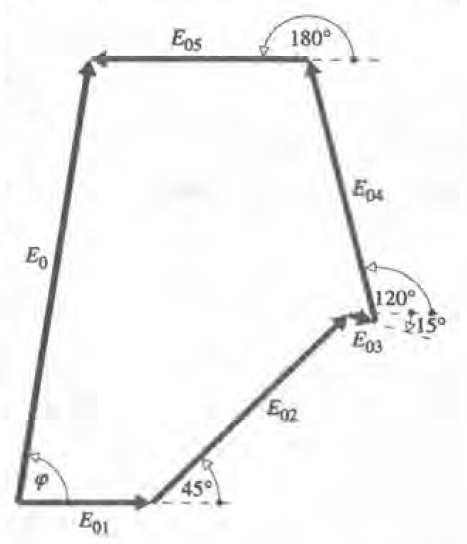
\includegraphics[width=0.3\linewidth]{figures/Phasor-Addition}
  \caption{Phasor Addition Method}
  \label{fig:}
\end{figure}

\section{Standing Waves}

\begin{equation*}
  \begin{aligned}
    & E_L = E_{0t} \sin \left( k x - \omega t \right) \\
    & E_R = E_{0t} \sin \left( k x - \omega t \right)
    & E = E_L + E_R
  \end{aligned}
\end{equation*}

\begin{equation*}
  \begin{aligned}
    \sin \alpha + \sin \beta = 2 \sin \dfrac{\alpha + \beta}{2} \cos \dfrac{\alpha - \beta}{2}  
  \end{aligned}
\end{equation*}

$\Rightarrow$

\begin{equation*}
  \begin{aligned}
    E = 2 E_{0t} \sin kx \cos \omega t
  \end{aligned}
\end{equation*}

\section{Addition of Waves of Different Frequency}

\begin{equation*}
  \left\{
    \begin{aligned}
      & E_1 = E_{01} \cos \left( k_1 x - \omega_1 t \right) \\
      & E_2 = E_{02} \cos \left( k_2 x - \omega_2 t \right) \\
      & E = E_1 + E_2
    \end{aligned}
  \right.
\end{equation*}

\begin{equation*}
  \begin{aligned}
    \cos \alpha + \cos \beta = 2 \cos \dfrac{\alpha + \beta}{2} \cos \dfrac{\alpha - \beta}{2}  
  \end{aligned}
\end{equation*}



$\Rightarrow$

\begin{equation*}
  \begin{aligned}
    E &= E_{01} \left[ \cos \left( k_1 x - \omega t \right) + \cos \left( k_2 x - \omega_2 t \right) \right] \\
    &= 2 E_{01} \cos \dfrac{1}{2} \left[ \left( k_1 + k_2 \right) x - \left( \omega_1 + \omega_2 \right) t \right] \times \cos \dfrac{1}{2} \left[ \left( k_1 - k_2 \right) x - \left( \omega_1 - \omega_2 \right) t \right]  
  \end{aligned}
\end{equation*}

Define

\begin{equation*}
  \begin{aligned}
    & \bar{\omega} = \dfrac{1}{2} \left( \omega_1 + \omega_2 \right) \\ 
    & \bar{k} = \dfrac{1}{2} \left( k_1 + k_2 \right) \\
  \end{aligned}
  \quad\quad\quad\quad
  \begin{aligned}
      & \omega_m = \dfrac{1}{2} \left( \omega_1 - \omega_2 \right) \\ 
      & k_m = \dfrac{1}{2} \left( k_1 - k_2 \right) 
  \end{aligned}
\end{equation*}

Then

\begin{equation*}
  \begin{aligned}
    E = 2 E_{01} \cos \left( k_m x - \omega_m t \right) \cos \left( \bar{k} x - \bar{\omega} t \right) = E_0 \left( x , t \right) \cos \left( \bar{k} x - \bar{\omega} t \right)
  \end{aligned}
\end{equation*}

Noted that

\begin{equation*}
  \begin{aligned}
    & \bar{\omega} = \dfrac{1}{2} \left( \omega_1 + \omega_2 \right) \\ 
    & \bar{k} = \dfrac{1}{2} \left( k_1 + k_2 \right) \\
  \end{aligned}
  \quad\quad \gg \quad\quad
  \begin{aligned}
      & \omega_m = \dfrac{1}{2} \left( \omega_1 - \omega_2 \right) \\ 
      & k_m = \dfrac{1}{2} \left( k_1 - k_2 \right) 
  \end{aligned}
\end{equation*}

$E_0 = 2 E_{01} \cos \left( k_m x - \omega_m t \right)$ varies far less frequently than $\cos \left( \bar{k} x - \bar{\omega} t \right)$

\begin{figure}[H]
  \centering
  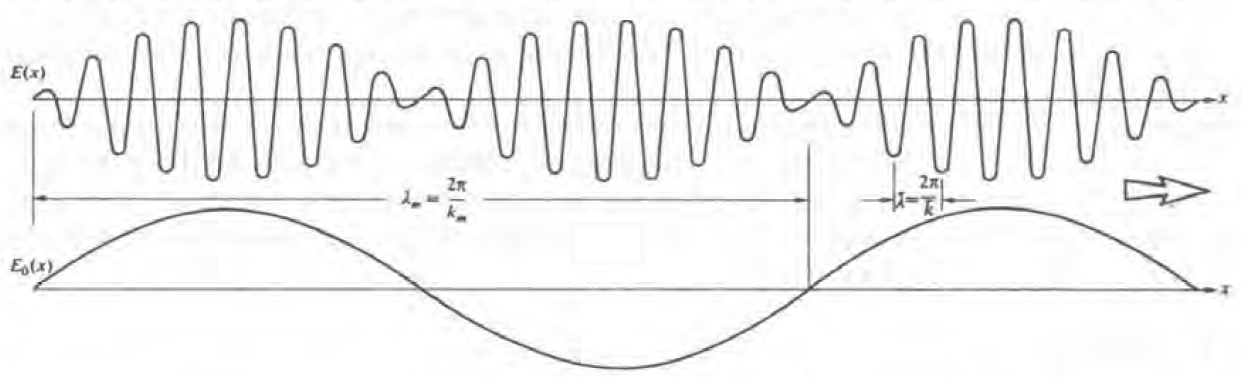
\includegraphics[width=\linewidth]{figures/Standing-Wave}
  \caption{Standing Wave}
  \label{fig:}
\end{figure}

\begin{table*}[h]
  \centering
  \begin{tabular}{|Sc|Sc|}
    \hline
    Beat Frequency (Time) & $2 \omega_m $ \\
    \hline
    Beat Frequency (Space) & $ 2 k_m $ \\
    \hline
  \end{tabular}
  \quad\quad\quad\quad
  \begin{tabular}{|Sc|Sc|}
    \hline
    Group Frequency & $v_g = \omega_m / k_m $ \\
    \hline
    Phase Velocity & $ v_p = \bar{\omega} / \bar{k}$ \\
    \hline
  \end{tabular}
\end{table*}

\section{Light in Dispersible Media}

\begin{table*}[h]
  \centering
  \begin{tabular}{|Sc|Sc|}
    \hline
    Average Phase Velocity & $\bar{v}_p = \dfrac{c}{\bar{n}} $ \\
    \hline
    Group Velocity & $v_g = \dfrac{c}{\bar{n}} \left( 1 + \dfrac{\bar{\lambda}}{\bar{n}} \dfrac{\Delta n}{\Delta \lambda}   \right) $ \\
    \hline
  \end{tabular}
  \quad\quad\quad\quad
  \begin{tabular}{|Sc|Sc|}
    \hline
    Normal Dispersion Media & $\bar{v}_p > v_g $ \\
    \hline
    Anomalous Dispersion Media & $ \bar{v}_p < v_g $ \\
    \hline
  \end{tabular}
\end{table*}


%%% Local Variables:
%%% mode: latex
%%% TeX-master: "Optics"
%%% End:



\end{document}